\documentclass{article}
\usepackage[utf8]{inputenc}
% Configuración de idioma español
\usepackage[spanish, es-tabla]{babel} 

% --- Matemáticas y Fuentes ---
\usepackage{amsmath}
\usepackage{amsfonts}
\usepackage{amssymb}

% --- Diseño y Formato ---
\usepackage{geometry}
\usepackage{indentfirst}
\usepackage{float}
\usepackage{booktabs}
\usepackage{subcaption}
\usepackage{graphicx}
\usepackage{xcolor}
\usepackage[most]{tcolorbox}
\usepackage{amsfonts}

% --- Algoritmos ---
\usepackage{algorithm}
\usepackage{algpseudocode}
\usepackage{pdflscape}
% --- Gráficos (TikZ y PGFPlots) ---
\usepackage{tikz}
\usepackage{tikz-3dplot}
\usepackage{pgfplots}
\usepackage[labelfont=bf, font=sf]{caption}
% Configuración de compatibilidad de PGFPlots
\pgfplotsset{compat=1.18} 

% Librerías de TikZ necesarias
\usetikzlibrary{positioning, shapes.geometric, arrows.meta, calc, backgrounds, fit, shadows, patterns, babel}


\raggedbottom
\setlength{\parskip}{1em}   
\setlength{\parindent}{0.75cm}
\geometry{
	a4paper,
	total={170mm,257mm},
	left=20mm,
	top=20mm,
}

\title{Trabajo: Técnicas de Reconocimiento de Patrones}
\author{Jorge Bengoa Pinedo \and Bogurad Barañski Barañska \and Sergio Izquierdo Morona }
\date{\today}

\begin{document}
	
	\maketitle
	
	\tableofcontents
	\newpage

	\section{Introducción a la clasificación de imágenes térmicas}
	
	Usamos la version YOLO v5 \cite{yolov5}
	Explicar el estado del arte un poco de que hay y tal.... redes tal, este otro tipo de clasificación
	\subsection{Redes Convolucionales...}
	\subsection{Metodología Yolo}
	\newpage
	\section{Fundamentos de funcionamiento de la red Yolo}
	A continuación se desarrrolla el funcionamiento de la red YOLO mediante la teoría de Marr para lo cuál es necesario describir el nivel implementacional y algoritmico. En este caso las redes neuronales artificiales se componen de 3 componentes que se describirán a continuación:
	\begin{itemize}
		\item Caracterización de la neurona.
		\item Definición de una topología de interconexión.
		\item Definición de unas reglas de entrenamiento.
	\end{itemize}
	
	\subsection{Neurona de la red Yolo}
	La unidad fundamental de procesamiento en la arquitectura YOLO es la capa convolucional (típica de las CNN). En esta sección se describe el funcionamiento de dicha operación, tomando como caso de estudio la capa de entrada, analizando tanto el entrenamiento específico realizado para imágenes térmicas como la implementación por defecto, tal como se ilustra en la Figura \ref{fig:neuronaInit}.
	\begin{figure}[H]
		\centering
		\shorthandoff{>} 
		
		\resizebox{\linewidth}{!}{
		\begin{tikzpicture}[
			font=\sffamily,
			>=Latex,
			% Define styles for the blocks
			block/.style={
				draw=blue!60!black, 
				fill=blue!5, 
				thick, 
				minimum height=1.5cm, 
				minimum width=2cm, 
				align=center,
				rounded corners=3pt,
				drop shadow
			},
			sum/.style={
				circle, 
				draw=black, 
				fill=white, 
				thick, 
				inner sep=0pt, 
				minimum size=0.8cm,
				drop shadow
			},
			label_text/.style={
				font=\footnotesize\color{gray!40!black}, 
				align=center
			},
			dim_text/.style={
				font=\small\bfseries\color{blue!40!black}
			}
			]
			
			% --- 1. INPUT ---
			\node (input) at (0,0) {\Large $X$};
			\node[label_text, above=0.2cm of input] {Input Image};
			\node[below=0.5cm of input] (dim_text) {$1 \times 3 \times 640 \times 640$};
			
			% Annotation for Batch/Channels
			\draw[->, gray, thin] (dim_text.south west) ++(0.2,-1.2) -- ++(0,1.3);
			\draw[->, gray, thin] (dim_text.south west) ++(0.8,-0.8) -- ++(0,0.9);
			\draw[->, gray, thin] (dim_text.south west) ++(1.6,-0.5) -- ++(0,0.6);			
			\draw[->, gray, thin] (dim_text.south west) ++(2.6,-0.8) -- ++(0,0.9);		
			
			\node[font=\small, anchor=north] at ([xshift=0.2cm,  yshift=-1.2cm]dim_text.south west) {Batch (Imágenes)};
			\node[font=\small, anchor=north] at ([xshift=0.8cm, yshift=-0.8cm]dim_text.south west) {Canales};
			\node[font=\small, anchor=north] at ([xshift=1.6cm,  yshift=-0.5cm]dim_text.south west) {Alto};
			\node[font=\small, anchor=north] at ([xshift=2.6cm,  yshift=-0.8cm]dim_text.south west) {Ancho};	
			
			% --- 2. CONVOLUTION BLOCK (W) ---
			\node[block, right=2.5cm of input] (conv) {\Large $W$};
			\draw[->, thick] (input) -- (conv);
			\node[above=0.8cm of conv, align=center] (w_dims) {
				$32 \times 3 \times 6 \times 6$
			};
			\draw[->, gray, thin] (w_dims.north west) ++(0.35, 1.2) -- ++(0,-1.2);
			\node[font=\small, anchor=south] at ([xshift=0.35cm, yshift=1.2cm]w_dims.north west) {Filtros};
			\draw[->, gray, thin] (w_dims.north west) ++(1.05, 0.6) -- ++(0,-0.6);
			\node[font=\small, anchor=south] at ([xshift=1.05cm, yshift=0.6cm]w_dims.north west) {Canales};
			\draw[decorate, decoration={brace, amplitude=3pt, mirror}, red!60!black, thick] 
			([xshift=1.35cm, yshift=0.1cm]w_dims.south west) -- 
			([xshift=2.35cm, yshift=0.1cm]w_dims.south west);
			\node[font=\small, red!60!black, anchor=north] at ([xshift=1.85cm, yshift=0.0cm]w_dims.south west) {Kernel};
			\draw[->, thick] (w_dims) -- (conv);
			\node[label_text, below=0.2cm of conv] {Convolución con los pesos $W$};
			
			
			% --- 3. SUMMATION (Bias) ---
			\node[sum, right=1.5cm of conv] (adder) {\Large $+$};
			
			% Arrow Conv -> Sum
			\draw[->, thick] (conv) -- node[above, font=\small] {$X*W$} (adder);
			
			% Bias Input
			\node[below=1.5cm of adder] (bias) {$b = (32 \times 1)$};
			\draw[decorate, decoration={brace, amplitude=4pt, mirror}, thick, black] 
			(bias.south west) -- (bias.south east) 
			node[midway, below=4pt, font=\small\normalfont, text=black] {Sesgo};
			\draw[->, thick] (bias) -- (adder);
			
			
			% --- 4. ACTIVATION (SiLU) ---
			\node[block, right=1.5cm of adder, minimum width=1.5cm] (silu) {SiLU\\ $\sigma(\cdot)$};
			\node[label_text, below=0.2cm of silu] {Función de activación};
			% Arrow Sum -> SiLU
			\draw[->, thick] (adder) -- (silu);
			
			
			% --- 5. OUTPUT ---
			\node[right=2.5cm of silu] (output) {\Large $f(X)$};
			
			% Arrow SiLU -> Output
			\draw[->, thick] (silu) -- (output);
			
			% Output Dimensions
			\node[dim_text, below=0.6cm of output, font=\small, text=black](dim_text_2) {$1 \times 32 \times 320 \times 320$};
			\node[label_text, above=0.2cm of output] {Espacio de características};
			
			% Annotation for Batch/Channels
			\draw[->, gray, thin] (dim_text_2.south west) ++(0.8,-1.2) -- ++(0,1.3);
			\draw[->, gray, thin] (dim_text_2.south west) ++(0.2,-0.8) -- ++(0,0.9);
			\draw[->, gray, thin] (dim_text_2.south west) ++(1.6,-0.5) -- ++(0,0.6);			
			\draw[->, gray, thin] (dim_text_2.south west) ++(2.6,-0.8) -- ++(0,0.9);		
			
			\node[font=\small, anchor=north] at ([xshift=0.2cm,  yshift=-0.8cm]dim_text_2.south west) {Batch };
			\node[font=\small, anchor=north] at ([xshift=0.8cm, yshift=-1.2cm]dim_text_2.south west) {Características};
			\node[font=\small, anchor=north] at ([xshift=1.6cm,  yshift=-0.5cm]dim_text_2.south west) {Alto};
			\node[font=\small, anchor=north] at ([xshift=2.6cm,  yshift=-0.8cm]dim_text_2.south west) {Ancho};	
			
		\end{tikzpicture}
		} % Close resizebox
		\caption{Estructura de la neurona a la entrada de la red YOLO.}
		\label{fig:neuronaInit}
	\end{figure}
	
	La operación de esta neurona convolucional está definida por los siguientes hiperparámetros:
	\begin{itemize}
		\item \textbf{Número de filtros (Características \(C_{out}\))}: Determinado por la primera dimensión del tensor de pesos. Define cuántos mapas de características se generarán.
		\item \textbf{Canales de entrada ($C_{in}$)}: Determinado por la segunda dimensión del tensor de pesos (e.g., 3 para RGB, 1 para imágenes térmicas).
		\item \textbf{Tamaño del Kernel ($k$)}: Define las dimensiones espaciales de la ventana de convolución (últimas dos dimensiones de los pesos). En la arquitectura YOLO analizada, se emplean principalmente los tamaños (6,6) para la entrada, y (3,3) o (1,1) para capas profundas.
		\item \textbf{Padding ($P$)}: Parámetro de relleno utilizado para controlar las dimensiones espaciales de la salida e indicar los bordes al llenarlos de ceros. En YOLO se utilizan típicamente valores de (2,2), (1,1), o (0,0).
		\item \textbf{Stride ($S$)}: Controla el paso o desplazamiento del filtro sobre la imagen. Un $S=1$ mueve el filtro píxel a píxel (preservando resolución), mientras que $S=2$ lo desplaza cada dos píxeles, reduciendo la dimensión espacial a la mita.
		\item \textbf{Dilatación ($d$)}: Controla la separación entre los puntos que analiza el kernel (también conocida como \textit{atrous convolution} cuando $d > 1$). En esta implementación de YOLO, el parámetro es (1,1), lo que indica una convolución estándar compacta sin huecos entre los elementos del kernel.
		\item \textbf{Agrupación ($g$)}: Controla la conectividad entre los canales de entrada y salida. Dado que en YOLO se utiliza $g=1$, se realiza una convolución estándar donde todos los canales de entrada contribuyen al cálculo de cada filtro de salida.
	\end{itemize}
	
	A partir de estos hiperparámetros, es posible determinar las dimensiones espaciales del mapa de características de salida. Dado que se contempla el factor de dilatación, se debe utilizar la relación generalizada descrita por \cite{conv}.
	\begin{equation} 
		\text{Salida} = \left\lfloor \frac{\text{Entrada} + 2 \cdot P - [k + (k-1)(d-1)]}{S} \right\rfloor + 1
	 \end{equation}
	
	En cuanto a la activación de cada neurona, el proceso consiste en aplicar la función SiLU (\textit{Sigmoid Linear Unit}) al resultado de la operación lineal (convolución más sesgo). Matemáticamente, la activación \(f(X)\) se expresa como:
	\begin{equation}
		f(X) = \underbrace{[(W * X) + b]}_{z} \cdot \sigma(\underbrace{[(W * X) + b]}_{z})
	\end{equation}
	\noindent donde \(\sigma(z) = \frac{1}{1+e^{-z}}\) es la función sigmoide logística. Se utiliza esta función de activación porque permite el calculo de gradientes y solo permite valores negativos pequeños para mejorar el flujo de gradientes \cite{silu,silu2}, se ilustra en la Figura \ref{fig:silu_plot}.

	\begin{figure}[H] 
		\centering
		\begin{tikzpicture}
			\begin{axis}[
				axis lines=middle,     
				xlabel={$z$},           
				ylabel={$SiLU(z)$},
				xlabel style={at={(ticklabel cs:1)}, anchor=north west},
				ylabel style={at={(ticklabel cs:1)}, anchor=south west},
				xmin=-4.5, xmax=4.5,
				ymin=-1.5, ymax=4.5,
				width=10cm, height=7cm, % Tamaño de la gráfica
				grid=major,
				grid style={line width=.1pt, draw=gray!20}
				]
				% EL COMANDO QUE FALLABA
				\addplot[color=blue!70!black, thick, mark=none, domain=-4.5:4.5, samples=100] 
				{x / (1 + exp(-x))};
				
				% Etiqueta manual dentro de la gráfica
				\node[color=blue!70!black, anchor=west] at (axis cs:1.5, 3) {$z \cdot \sigma(z)$};
				
				% Mínimo local (decoración)
				\draw[dashed, help lines] (axis cs:-1.28, 0) -- (axis cs:-1.28, -0.278);
			\end{axis}
		\end{tikzpicture}
		\caption{Representación gráfica de la función de activación SiLU.}
		\label{fig:silu_plot}
	\end{figure}
	
	Por otro lado, la operación de convolución discreta 2D ($W*X$) en el contexto de aprendizaje profundo se implementa técnicamente como una correlación cruzada (sin voltear el kernel) pues solo se busca conocer los pesos y no aplicar un filtro con una topología concreta. Para un filtro de salida específico ($c_{out}$) en la posición espacial $(h, w)$, la operación se define formalmente como \cite{conv}:	
	\begin{equation}
		(W * X)(c_{out}, h, w) = \sum_{l=0}^{\frac{C_{in}}{g}-1} \sum_{i=0}^{K_H-1} \sum_{j=0}^{K_W-1} W(c_{out}, l, i, j) \cdot X(l, h \cdot S + i \cdot d , w \cdot S + j \cdot d)
	\end{equation}
	\newpage
	\subsection{Topología de la red}
	En esta sección tras analizar los artículos principales de los creadores de Yolo \cite{redmon2016lookonceunifiedrealtime}\cite{redmon2016yolo9000betterfasterstronger}\cite{redmon2018yolov3incrementalimprovement}\cite{bochkovskiy2020yolov4optimalspeedaccuracy} y el diagrama de la red mediante la herramienta \textit{Netron} donde se introduce la red en formato \textit{.onnx} y se analiza su diagrama que tiene una forma similar al de la figura \ref{fig:fotoneutron}.
	
	\begin{figure}[H]
		\centering
		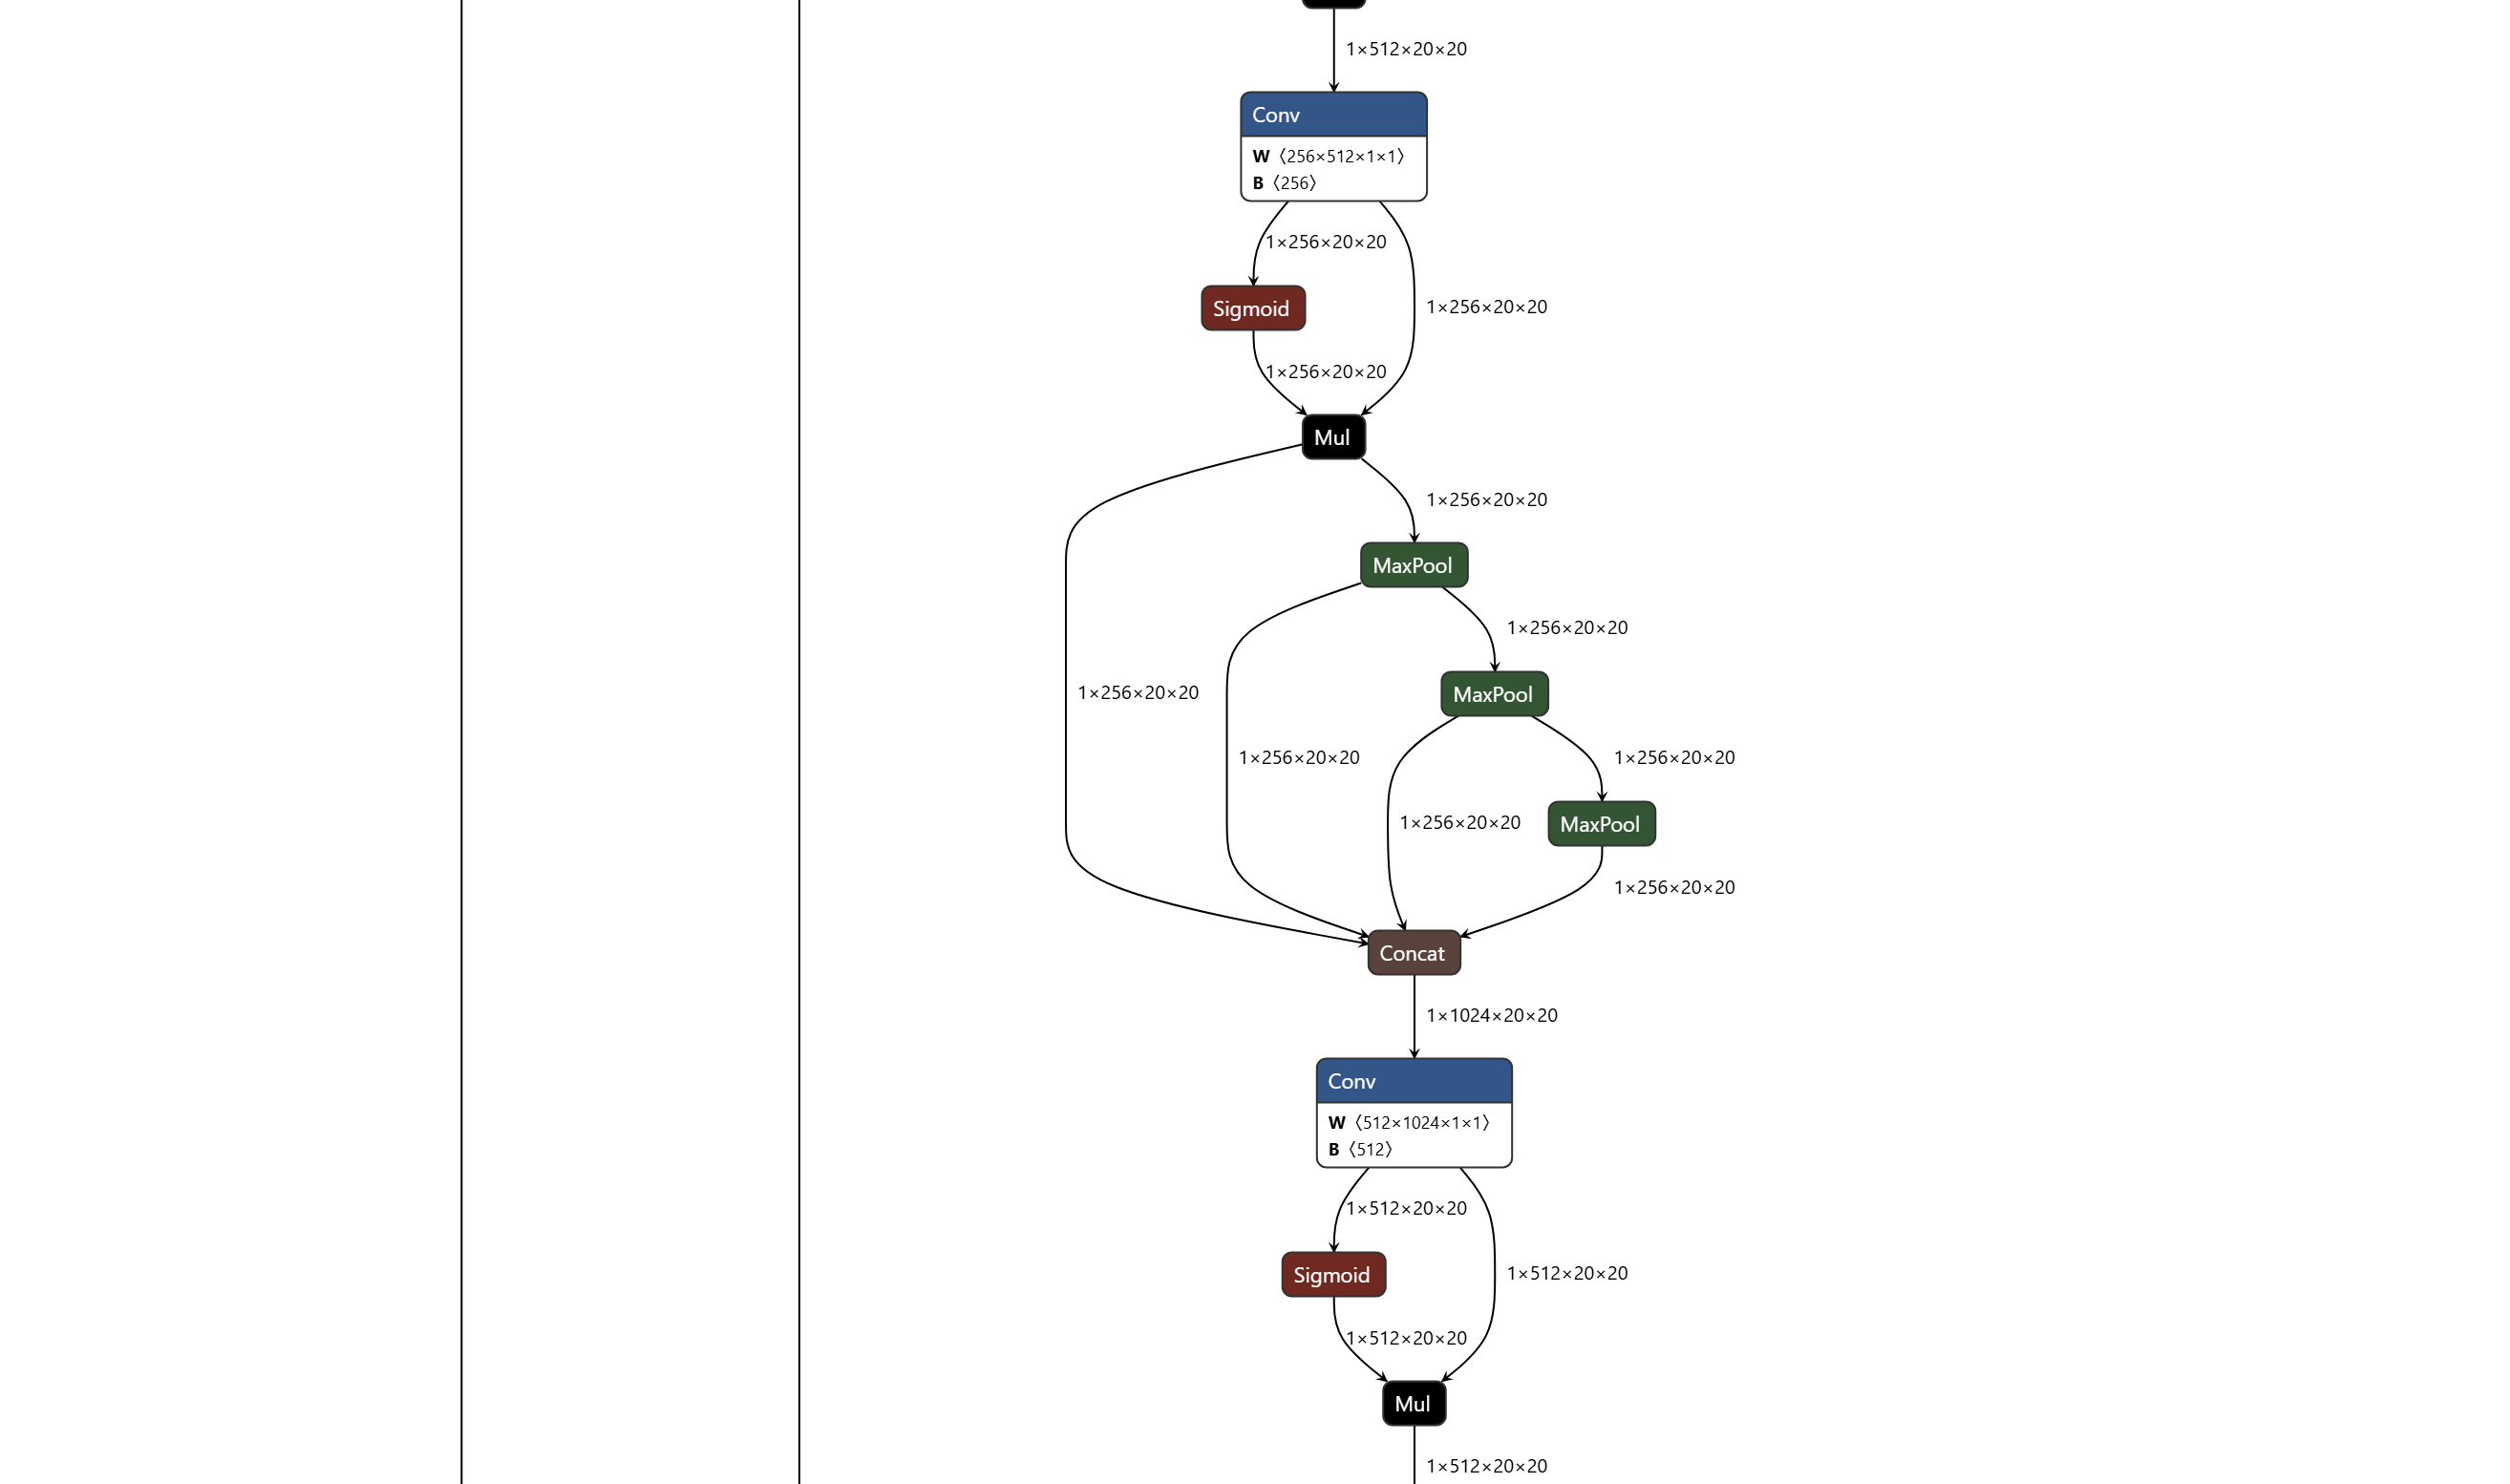
\includegraphics[width=0.7\linewidth]{FotoNeutron}
		\caption{Ejemplo de parte de la red Yolo en la aplicación \textit{Netron}.}
		\label{fig:fotoneutron}
	\end{figure}
	
	Uno de los bloques que más se repite a lo largo de la arquitectura de la red Yolo es el bloque ResNet, cuya estructura se encuentra representada en la figura \ref{fig:standard_bottleneck}. La filosofía detrás del diseño de este bloque viene detallada en el artículo  \cite{he2015deepresiduallearningimage}, y su objetivo principal se mejorar el rendimiento de las redes neuronales profundas cuando se acumulan múltiples capas.
	\newline
	
	La problemática surge durante el entrenamiento: al acumular múltiples capas consecutivas, los gradientes tienden a explotar. Antes de la existencia de este bloque, esto se mitigaba mediante la normalización en capas intermedias, pero aun así se observaba una degradación en la convergencia. Para entender esta degradación, se puede entender la operación de convolución como una aplicación identidad con cierto ruido superpuesto que representa las características a extraer. Por tanto, mediante una conexión lineal directa se optimiza el comportamiento del método de optimización utilizado, mejorando así la convergencia. 
	\newline
	
	La premisa de que los bloques se comportan como aplicaciones lineales con ruido se demuestra empíricamente en el propio artículo \cite{he2015deepresiduallearningimage}. Aunque se trata más de una heurística que de un argumento formal, en casos reales, como el de la figura \ref{fig:fotoresnet}, presenta un mejor comportamiento que simplemente acumular capas, y solo sería problemático si el objetivo del bloque fuera aproximar la función nula.
	\newline
	
	La interpretación del bloque ResNet como una aplicación lineal con ruido se deduce fácilmente a partir de las ecuaciones del modelo:
	\begin{equation}
		y=\mathcal{H}(x)=\mathcal{F}(x)+x
	\end{equation}
	donde \(y\) es la salida de aplicar \(\mathcal{H}\) a la entrada \(x\) que se descompone entre una función que representa la convolución \(\mathcal{F}(x)\) y la aplicación líneal directa. Por tanto, se puede asemejar el funcionamiento de las capas convolucionales como un extractor del ruido o características. 
	\newline
	
	Profundizando en el detalle del propio bloque, este está formado por dos capas, donde la primera se encarga de procesar los canales para que la segunda simplemente extraiga las características de los anteriores.
	
	
	\begin{figure}[H]
		\centering
		
		% --- TikZ Setup ---
		\begin{tikzpicture}[
			node distance=1.5cm,
			% --- Styles ---
			cvblock/.style={
				rectangle, draw, rounded corners, fill=cyan!10, drop shadow,
				minimum width=1.2cm, minimum height=1.2cm, align=center, font=\bfseries\sffamily\scriptsize
			},
			% Rhombus Style for Sumator
			sumnode/.style={
				diamond, draw, fill=green!10, drop shadow,
				minimum width=1.0cm, minimum height=1.0cm, align=center, font=\bfseries\sffamily\large, inner sep=0pt
			},
			line/.style={
				draw, -Latex, thick, color=darkgray
			},
			dimlabel/.style={
				font=\sffamily\tiny, color=gray, align=center, auto
			}
			]
			
			% --- 1. Input Node (Invisible start point) ---
			\node (input_start) {};
			
			% --- 2. Main Processing Branch (Top) ---
			% First CV
			\node [cvblock, right=2cm of input_start] (cv1) {CV\\$W_{A}$};
			
			% Second CV
			\node [cvblock, right=1.2cm of cv1] (cv2) {CV\\$W_{B}$};
			
			% Sumator (Rhombus)
			\node [sumnode, right=1.2cm of cv2, label=below:\sffamily\scriptsize] (sigma) {$\Sigma$};
			
			% --- 3. Connections & Shortcut ---
			
			% Input Line
			\draw [line] (input_start) -- (cv1.west);
			
			% Label Input Size
			\node [dimlabel, above] at ($(input_start)!0.5!(cv1.west)$) {Tamaño Entrada\\$C \times H \times W$};
			
			% Internal Connections (Main Branch)
			\draw [line] (cv1) -- node[dimlabel, above] {} (cv2);
			\draw [line] (cv2) -- (sigma.west);
			
			% --- The Residual Shortcut (The "Loop") ---
			% Define a split point before CV1
			\coordinate (split_point) at ($(cv1.west) + (-1.0, 0)$);
			
			% Define the target at the BOTTOM of the diamond
			\coordinate (sigma_bottom) at (sigma.south);
			
			% Draw Shortcut Line:
			% 1. Start at split point
			% 2. Go Down (vertical)
			% 3. Go Right (horizontal) until under the sigma
			% 4. Go Up into the sigma
			% --- The Residual Shortcut (The "Loop") ---
			\coordinate (split_point) at ($(cv1.west) + (-1.0, 0)$);
			\coordinate (sigma_bottom) at (sigma.south);
			
			% 1. The Line (Clean)
			\draw [line] (split_point) -- ++(0, -1.8) -| (sigma_bottom);
			
			% 2. The Text (Separated)
			% Logic: Located halfway (0.5) horizontally between start and end, 
			% and shifted down 1.8cm to match the line's depth.
			\node [font=\sffamily\tiny, color=gray, below, yshift=-2pt] 
			at ($(split_point)!0.5!(sigma) + (0, -1.8)$) 
			{Identidad (Residuos)};
			

			% Dot
			\fill [darkgray] (split_point) circle (2pt);
			% Add the visual "dot" at the split point for clarity
			\fill [darkgray] (split_point) circle (2pt);
			
			% --- 4. Final Output ---
			\node [right=1.5cm of sigma] (output_end) {};
			\draw [line] (sigma.east) -- (output_end);
			
			% Label Output Preservation
			\node [dimlabel, above] at ($(sigma.east)!0.5!(output_end)$) {Tamaño Salida\\$C \times H \times W$\\(Preservada)};
			
			% --- 5. Legend ---
			\node [draw, dashed, fill=white, rounded corners, 
			font=\sffamily\scriptsize, align=left, anchor=north,
			% CHANGE THE NUMBERS BELOW TO MOVE THE BOX: (X, Y)
			at={($(cv2) + (-0.5, -2.2)$)}] {
				\textbf{Leyenda:}\\
				\textbf{CV}: Neurona convolucional\\
				\textbf{$\Sigma$}: Suma elemento a elemento\\
				\textbf{C}: Número de canales\\
				\textbf{H,W}: Ancho y alto de los mapas de características.\\
				$W_{A}=\{C, C, 1, 1\}$: Reduce/Procesa canales (1x1)\\
				$W_{B}=\{C, C, 3, 3\}$: Extracción características (3x3)
			};
			
		\end{tikzpicture}
		
		% --- Caption serves as Title ---
		\caption{Arquitectura de un bloque ResNet.}
		\label{fig:standard_bottleneck}
	\end{figure}
	
	\begin{figure}[H]
		\centering
		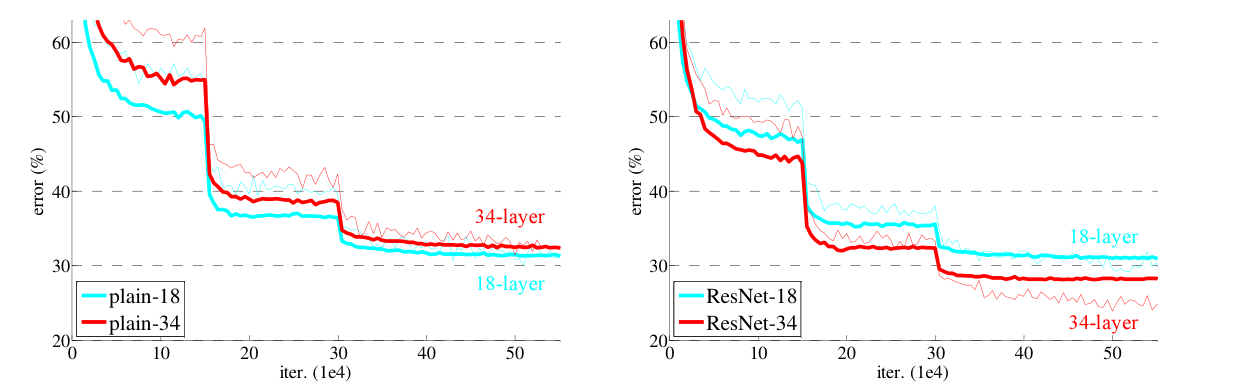
\includegraphics[width=0.7\linewidth]{fotoResNet}
		\caption{Representación del error de entrenamiento en función del número de capas. A la izquierda se representa una arquitectura con capas apiladas y a la derecha una arquitectura de capas apiladas utilizando el bloque ResNet.}
		\label{fig:fotoresnet}
	\end{figure}
	
	
	Para elaborar el bloque \ref{fig:csp_bottleneck} se usa el artículo \cite{wang2019cspnetnewbackboneenhance}
	\begin{figure}[H]
		\centering
		\resizebox{\linewidth}{!}{
		% --- TikZ Setup ---
		\begin{tikzpicture}[
			node distance=1.5cm,
			% --- Styles ---
			cvblock/.style={
				rectangle, draw, rounded corners, fill=cyan!10, drop shadow,
				minimum width=1.2cm, minimum height=1.2cm, align=center, font=\bfseries\sffamily\scriptsize
			},
			concatblock/.style={
				rectangle, draw, fill=orange!20, drop shadow,
				minimum width=1cm, minimum height=3.5cm, align=center, font=\bfseries\sffamily\small
			},
			line/.style={
				draw, -Latex, thick, color=darkgray
			},
			dimlabel/.style={
				font=\sffamily\tiny, color=gray, align=center, auto
			}
			]
			
			% --- 1. Entry Concatenator ---
			\node [concatblock, label=below:\sffamily\scriptsize In Concat] (concat_in) {CONCAT};
			
			% Inputs to Entry Concat
			\draw [line] ($(concat_in.west) + (-2, 0.5)$) -- node[above, font=\tiny] {In 1} ($(concat_in.west) + (0, 0.5)$);
			\draw [line] ($(concat_in.west) + (-2, -0.5)$) -- node[below, font=\tiny] {In 2} ($(concat_in.west) + (0, -0.5)$);
			
			% --- 2. Top Branch (Main Processing: 3 CVs) ---
			% Position relative to entry concat
			\node [cvblock, above right=0.0cm and 1.5cm of concat_in] (top1) {CV\\$W_{1}$};
			\node [cvblock, right=0.8cm of top1] (top2) {CV\\$W_{2}$};
			\node [cvblock, right=0.8cm of top2] (top3) {CV\\$W_{3}$};
			
			% --- 3. Bottom Branch (Shortcut: 1 CV) ---
			% Positioned centrally below the top chain for symmetry
			% We align it horizontally with top2 so it looks balanced
			\node [cvblock, below=3.5cm of top2] (bot1) {CV\\$W_{1}$};
			
			% --- Connections from Entry Concat to Branches ---
			\coordinate (split_point) at ($(concat_in.east) + (0.5, 0)$);
			
			% 1. Draw the line (Clean, no text)
			\draw [line] (concat_in.east) -- (split_point);
			
			% 2. Draw the text (Separately)
			% We place it exactly halfway (0.5) between concat_in and split_point
			\node [dimlabel, above, yshift=-6pt] at ($(concat_in.east)!2.6!(split_point)$) {$2C \times H \times W$};
			
			\node [dimlabel, above, yshift=-8pt] at ($(concat_in.east)!-6!(split_point)$) {Tamaño Entrada\\$C \times H \times W$};
			
			% To Top (No text)
			\draw [line] (split_point) |- (top1.west);
			
			% To Bottom (No text)
			\draw [line] (split_point) |- (bot1.west);
			
			% --- Connections within branches ---
			% Top chain
			\draw [line] (top1) -- (top2);
			\draw [line] (top2) -- (top3);
			
			% --- 4. Output Concatenator ---
			\node [concatblock, right=9cm of concat_in, label=below:\sffamily\scriptsize Out Concat] (concat_out) {CONCAT};
			

			
			% FIX: Define a shared vertical axis for the bend (0.8cm to the right of top3)
			% This ensures both lines turn at the exact same X-coordinate
			\coordinate (turn_axis) at ($(top3.east) + (0.8, 0)$);
			
			% Connect Top Branch (Path 1)
			\coordinate (in_top) at ($(concat_out.west) + (0, 0.6)$);
			
			% Draw: (Start) -- (Go to Axis) |- (Target)
			% The syntax (source -| turn_axis) finds the intersection point (axis X, source Y)
			\draw [line] (top3.east) -- (top3.east -| turn_axis) |- (in_top) node[left, font=\tiny, xshift=-2pt,yshift=-5pt] {(1)}; 
			
			% Connect Bottom Branch (Path 2)
			\coordinate (in_bot) at ($(concat_out.west) + (0, -0.6)$);
			
			% Draw: Same logic, it will extend the line further to hit the same axis
			\draw [line] (bot1.east) -- (bot1.east -| turn_axis) |- (in_bot) node[left, font=\tiny, xshift=-2pt,yshift=5pt] {(2)};
			% --- Legend / Info Box ---
			% --- 5. Final Transition & Output ---
			% Add the final CV block after Concat
			\node [cvblock, right=1.0cm of concat_out] (final_cv) {CV\\$W_{4}$};
			\draw [line] (concat_out.east) -- (final_cv.west);
			
			% Draw the final outgoing line
			\node [right=1.5cm of final_cv] (final_out) {};
			\draw [line] (final_cv.east) -- (final_out);
			
			% Label the preservation of size at the very end
			\node [dimlabel, above] at ($(final_cv.east)!0.5!(final_out)$) {Tamaño Salida\\$C \times H \times W$\\(Preservada)};
			
			\node [draw, dashed, fill=white, rounded corners, below=0.5cm of bot1, font=\sffamily\scriptsize, align=left] {
				\textbf{Leyenda:}\\
				\textbf{CV}: Neurona convolucional\\
				\textbf{Concat}: Concatenador de cadenas\\
				\textbf{C}: Número de canales\\
				\textbf{H,W}: Ancho y alto de los mapas de características.\\
				$W_{1}=\{C/2,2C,1,1\}$: Pesos neuronas de entrada para ...\\
				$W_{2}=\{C/2,C/2,1,1\}$: Pesos neurona de...\\
				$W_{3}=\{C/2,C/2,3,3\}$: Pesos neurona de...\\
				$W_{4}=\{C,C,1,1\}$: Pesos neurona de salida para...
			};
			
		\end{tikzpicture}
		}
		% --- Caption serves as Title ---
		\caption{Architecture of the CSP (YOLOv5 C3 Module)}
		\label{fig:csp_bottleneck}
	\end{figure}
	
	Para elaborar el bloque \ref{fig:c3_final} se usa el artículo \cite{wang2019cspnetnewbackboneenhance}
	\begin{figure}[H]
		\centering
		\resizebox{\linewidth}{!}{
		% --- TikZ Setup ---
		\begin{tikzpicture}[
			node distance=1.5cm,
			% --- Styles ---
			cvblock/.style={
				rectangle, draw, rounded corners, fill=cyan!10, drop shadow,
				minimum width=1.2cm, minimum height=1.2cm, align=center, font=\bfseries\sffamily\scriptsize
			},
			resnetblock/.style={
				rectangle, draw, fill=yellow!20, rounded corners, drop shadow,
				minimum width=1.5cm, minimum height=1.2cm, align=center, font=\bfseries\sffamily\scriptsize
			},
			concatblock/.style={
				rectangle, draw, fill=orange!20, drop shadow,
				minimum width=1cm, minimum height=3.5cm, align=center, font=\bfseries\sffamily\small
			},
			line/.style={
				draw, -Latex, thick, color=darkgray
			},
			dimlabel/.style={
				font=\sffamily\tiny, color=gray, align=center, auto
			}
			]
			
			% --- 1. Entrada y CV Inicial ---
			\node (input_start) {};
			
			% CV de Entrada (NUEVO)
			\node [cvblock] (cv_in) at (0,0) {CV\\$W_{1}$};
			
			% Línea desde "nada" hasta CV in
			\draw [line] ($(cv_in.west) + (-1.5, 0)$) -- node[dimlabel, above] {} (cv_in.west);
			\node [font=\sffamily\tiny, color=gray, below] 
			at ($(split_point)!0.5!(sigma_bottom) + (-5.8, 0.75)$) 
			{$C\times H \times W$};
			
			\node [font=\sffamily\tiny, color=gray, below] 
			at ($(split_point)!0.5!(sigma_bottom) + (-2.8, 0.75)$) 
			{$2C\times H/2 \times W/2$};
			% --- 2. Punto de División (Split) ---
			% El punto de split está justo a la salida de la CV de entrada
			\coordinate (split_point) at ($(cv_in.east) + (2.0, 0)$);
			\draw [line] (cv_in.east) -- (split_point);
			
			
			% --- 3. Rama Superior (Procesamiento) ---
			% CV Rama Superior
			\node [cvblock, above right=0.5cm and 1.0cm of split_point] (top_cv) {CV\\$W_{2}$};
			
			% ResNet Bloque 1
			\node [resnetblock, right=0.8cm of top_cv] (res1) {Bloque\\ResNet};
			
			% ResNet Bloque 2
			\node [resnetblock, right=1.0cm of res1] (res2) {Bloque\\ResNet};
			
			% Conexiones Superiores
			\draw [line] (split_point) |- (top_cv.west);
			\draw [line] (top_cv) -- (res1);
			
			% FLECHA PUNTEADA ENTRE RESNETS (NUEVO)
			\draw [line, dashed] (res1) -- (res2);
			
			% Llave indicando k veces
			\draw [decorate, decoration={brace, amplitude=6pt, raise=4pt}, thick, color=darkgray]
			(res1.north west) -- (res2.north east)
			node [midway, above=10pt, font=\sffamily\scriptsize\bfseries] {$\times k$ veces};
			
			
			% --- 4. Rama Inferior (Atajo) ---
			% CV Rama Inferior
			\node [cvblock, below right=0.5cm and 1.0cm of split_point] (bot_cv) {CV\\$W_{2}$};
			
			% Conexión Inferior
			\draw [line] (split_point) |- (bot_cv.west);
			
			
			% --- 5. Concatenación de Salida ---
			\node [concatblock, right=1.5cm of res2, yshift=-1.1cm, label=below:\sffamily\scriptsize ] (concat_out) {CONCAT};
			
			% Ejes de giro para flechas simétricas
			\coordinate (turn_axis) at ($(res2.east) + (0.8, 0)$);
			
			% Conexión Superior (1)
			\coordinate (in_top) at ($(concat_out.west) + (0, 0.6)$);
			\draw [line] (res2.east) -- (res2.east -| turn_axis) |- (in_top) node[left, font=\tiny, xshift=-2pt,yshift=-5pt] {(1)}; 
			
			% Conexión Inferior (2)
			\coordinate (in_bot) at ($(concat_out.west) + (0, -0.6)$);
			\draw [line] (bot_cv.east) -- (bot_cv.east -| turn_axis) |- (in_bot) node[left, font=\tiny, xshift=-2pt,yshift=5pt] {(2)};
			
			
			% --- 6. CV Final y Salida ---
			\node [cvblock, right=1.0cm of concat_out] (final_cv) {CV\\$W_{3}$};
			\draw [line] (concat_out.east) -- (final_cv.west);
			
			\node [right=1.5cm of final_cv] (final_out) {};
			\draw [line] (final_cv.east) -- (final_out);
			\node [dimlabel, above] at ($(final_cv.east)!0.7!(final_out)$) {Salida\\$2C\times H/2 \times W/2$};
			
			
			% --- 7. Leyenda ---
			\node [draw, dashed, fill=white, rounded corners, font=\sffamily\scriptsize, align=left, anchor=north, at={($(bot_cv) + (2.5, -1.3)$)}] {
				\textbf{Leyenda:}\\
				\textbf{CV}:  Neurona convolucional\\
				\textbf{Bloque ResNet}: Módulo residual repetido\\
				\textbf{C}: Número de canales\\
				\textbf{H,W}: Ancho y alto de los mapas de características.\\
				$W_{1}=\{2C,C,3,3\}$: Pesos neuronas de entrada para ...\\
				$W_{2}=\{C,2C,1,1\}$: Pesos neurona de...\\
				$W_{3}=\{2C,2C,1,1\}$: Pesos neurona de salida para...
			};
		
		\end{tikzpicture}
		}
		\caption{Arquitectura del Módulo CSPResNe(X)t o C3-k}
		\label{fig:c3_final}
	\end{figure}
	
	
	To enlarge the receptive field and fuse features at different scales, we employ the Spatial Pyramid Pooling - Fast (SPPF) module. This is an optimized implementation of the original Spatial Pyramid Pooling (SPP) proposed by He et al. \cite{He_2014}.While the original SPP processes features through parallel pooling windows of sizes $k=\{1, 5, 9, 13\}$, SPPF achieves the same mathematical result by sequentially passing the input through multiple $5\times5$ max-pooling layers. This sequential structure, introduced in the YOLOv5 architecture \cite{yolov5}, significantly reduces computational latency while preserving the multi-scale feature fusion capability." \ref{fig:sppf_cascade} 
	\begin{figure}[H]
		\centering
		
		% --- PROTECCIÓN DE BABEL (Importante para evitar el crash) ---
		\shorthandoff{<}
		\shorthandoff{>}
		
			\resizebox{\linewidth}{!}{
			\begin{tikzpicture}[
				node distance=1.0cm,
				% --- ESTILOS ---
				cvblock/.style={
					rectangle, draw, rounded corners, fill=cyan!10, drop shadow,
					minimum width=1.5cm, minimum height=1.2cm, align=center, font=\bfseries\sffamily\scriptsize
				},
				mpblock/.style={
					rectangle, draw, rounded corners, fill=red!15, drop shadow,
					minimum width=1.5cm, minimum height=1.2cm, align=center, font=\bfseries\sffamily\scriptsize
				},
				concatblock/.style={
					rectangle, draw, fill=orange!20, drop shadow,
					minimum width=1.2cm, minimum height=7.5cm, align=center, font=\bfseries\sffamily\small
				},
				line/.style={
					draw, -Latex, thick, color=darkgray
				},
				dimlabel/.style={
					font=\sffamily\tiny, color=gray, align=center, auto
				},
				dot/.style={
					circle, fill=darkgray, inner sep=0pt, minimum size=4pt
				}
				]
				
				% --- 1. La Pila Vertical (The Stack) ---
				% Alineamos todos los bloques uno debajo del otro
				
				% Bloque 1: CV
				\node [cvblock] (cv_in) {CV\\$W_{1}$};
				\draw [line] ($(cv_in.west) + (-2.0, 0)$) -- node[dimlabel, above] {Entrada\\$C \times H \times W$} (cv_in.west);
				
				% Bloque 2: MP1
				\node [mpblock, below=1.0cm of cv_in, xshift=2.0cm] (mp1) {MP\\$k=5$};
				
				% Bloque 3: MP2
				\node [mpblock, below=1.0cm of mp1, xshift=2.0cm] (mp2) {MP\\$k=5$};
				
				% Bloque 4: MP3
				\node [mpblock, below=1.0cm of mp2, xshift=2.0cm] (mp3) {MP\\$k=5$};
				
				
				% --- 2. El Concat (Alta torre a la derecha) ---
				% Lo posicionamos a la derecha del conjunto
				\node [concatblock, right=4.5cm of $(cv_in)!0.5!(mp3)$] (concat_out) {{CONCAT}};
				
				
				% --- 3. Las Conexiones "Cascada" (La Escalera) ---
				
				% Definimos los 4 puertos de entrada en el Concat alineados horizontalmente con cada bloque
				% Usamos la sintaxis (origen -| destino) para que queden perfectamente rectos
				\coordinate (port1) at (cv_in -| concat_out.west);
				\coordinate (port2) at (mp1 -| concat_out.west);
				\coordinate (port3) at (mp2 -| concat_out.west);
				\coordinate (port4) at (mp3 -| concat_out.west);
				
				
				% --- NIVEL 1: Salida de CV ---
				% 1. Línea Recta al Concat
				\draw [line] (cv_in.east) -- (port1) node[midway, above, font=\tiny] {(1)};
				
				% 2. La Bajada (Escalera) hacia MP1
				% Ponemos un punto (dot) en la línea recta y bajamos hacia el NORTE de MP1
				\coordinate (split1) at ($(mp1.north) + (0, 1.6)$); 
				\node [dot] at (split1) {};
				
				% CHANGE: Use .east instead of .north
				\draw [line] (split1) -- (mp1.north);
				
				
				% --- NIVEL 2: Salida de MP1 ---
				% 1. Línea Recta al Concat
				\draw [line] (mp1.east) -- (port2) node[midway, above, font=\tiny] {(2)};
				
				% 2. La Bajada hacia MP2
				\coordinate (split2) at ($(mp2.north) + (0, 1.6)$);
				\node [dot] at (split2) {};
				\draw [line] (split2) -- (mp2.north);
				
				
				% --- NIVEL 3: Salida de MP2 ---
				% 1. Línea Recta al Concat
				\draw [line] (mp2.east) -- (port3) node[midway, above, font=\tiny] {(3)};
				
				% 2. La Bajada hacia MP3
				\coordinate (split3) at ($(mp3.north) + (0, 1.6)$);
				\node [dot] at (split3) {};
				\draw [line] (split3) -- (mp3.north);
				
				
				% --- NIVEL 4: Salida de MP3 (Última) ---
				% Solo va recta al Concat
				\draw [line] (mp3.east) -- (port4) node[midway, above, font=\tiny] {(4)};
				
				
				% --- 4. Salida Final ---
				\node [cvblock, right=1.0cm of concat_out] (cv_out) {CV\\$W_{2}$};
				\draw [line] (concat_out.east) -- (cv_out.west);
				
				\node [right=1.5cm of cv_out] (end_point) {};
				\draw [line] (cv_out.east) -- (end_point);
				\node [dimlabel, above] at ($(cv_out.east)!0.5!(end_point)$) {Salida\\$C \times H \times W$};
				
				
				% --- 5. Leyenda ---
				\node [draw, dashed, fill=white, rounded corners, font=\sffamily\scriptsize, align=left, anchor=north west, at={($(mp3.south) + (-8.5, 1)$)}] {
					\textbf{Leyenda:}\\
					\textbf{CV}: Neurona convolucional\\
					\textbf{Concat}: Concatenador de cadenas\\
					\textbf{MP}: MaxPool ($k=5$)\\
					\textbf{C}: Número de canales\\
					\textbf{H,W}: Ancho y alto de los mapas de características.\\
					$W_{1}=\{C/2,C,1,1\}$: Pesos neuronas de entrada para ...\\
					$W_{2}=\{C,2C,1,1\}$: Pesos neurona de salida para...
				};
				
			\end{tikzpicture}
		}
		\caption{Arquitectura SPP en Cascada}
		\label{fig:sppf_cascade}
	\end{figure}
	
	
	La estructura de la cabeza \ref{fig:yolo_head_detail} puede explicarse directamente a través de los artículos de Yolo
	\begin{figure}[H]
		\centering
		\shorthandoff{<}\shorthandoff{>}
		
		\resizebox{\linewidth}{!}{
			\begin{tikzpicture}[
				node distance=1.5cm and 2.0cm, 
				% --- ESTILOS ---
				cvblock/.style={
					rectangle, draw, rounded corners, fill=cyan!10, drop shadow,
					minimum width=2.0cm, minimum height=1.2cm, align=center, font=\bfseries\sffamily\scriptsize
				},
				concatblock/.style={
					rectangle, draw, fill=orange!20, drop shadow,
					minimum width=1.2cm, minimum height=4.5cm, align=center, font=\bfseries\sffamily\small
				},
				opnode/.style={
					circle, draw, fill=gray!10, drop shadow, thick,
					minimum size=1.2cm, align=center, font=\bfseries\sffamily\large
				},
				line/.style={
					draw, -Latex, thick, color=darkgray, rounded corners=5pt
				},
				dimlabel/.style={
					font=\sffamily\tiny, color=darkgray, align=center, auto, fill=white, inner sep=1pt
				},
				dot/.style={
					circle, fill=darkgray, inner sep=0pt, minimum size=4pt
				}
				]
				
				% ==========================================
				% 1. Entrada y Convolución Inicial (Wi)
				% ==========================================
				\node (input_i) at (0,0) {\Large $i$};
				\node [opnode, right=1.0cm of input_i] (wi_node) {$W_i$};
				\draw [line] (input_i) -- (wi_node);
				
				% ==========================================
				% 2. Primer Reshape y Activación
				% ==========================================
				\node [cvblock, right=3.0cm of wi_node] (reshape1) {Reshape};
				\draw [line] (wi_node) -- node[dimlabel] {$1 \times 255 \times H \times W$} (reshape1);
				
				\node [opnode, right=1.5cm of reshape1] (sigma_node) {$\sigma$};
				\draw [line] (reshape1) -- coordinate (mid) (sigma_node);
				\draw [thin, darkgray] (mid) -- ++(0, 0.6) node[dimlabel, anchor=south] {$3 \times H \times W \times 85$};
				
				% ==========================================
				% 3. División en 3 Ramas y Primer Concat
				% ==========================================
				\node [concatblock, right=6.0cm of sigma_node] (concat1) {Concat};
				
				% --- MODIFICATION START ---
				
				% 1. Define Coords block to span Middle (y=0) and Bottom (y=-1.5)
				% We position it halfway horizontally, and shift it down by 0.75cm vertically
				% We also increase height to 2.5cm to cover both "lanes"
				\node [cvblock, minimum height=2.8cm] (coords) at ($(sigma_node)!0.5!(concat1) + (0, -0.75)$) {Coords};
				
				% 2. Split Point
				\coordinate (split_sigma) at ($(sigma_node.east) + (1.0, 0)$);
				\draw [line] (sigma_node) -- (split_sigma);
				\node [dot] at (split_sigma) {};
				
				% 3. Concat Inputs
				\coordinate (concat1_in1) at ($(concat1.west) + (0, 1.5)$);
				\coordinate (concat1_in2) at (concat1.west); % Middle input
				\coordinate (concat1_in3) at ($(concat1.west) + (0, -1.5)$); % Bottom input
				
				% --- Branch 1: Top (Classes) ---
				\draw [line] (split_sigma) |- (concat1_in1) 
				node[dimlabel, pos=0.7] {$3 \times H \times W \times 81$} 
				node[at end, left, font=\tiny, xshift=-3pt,yshift=5] {1};
				
				% --- Branches 2 & 3: Coords & Objectness (Going through the big block) ---
				
				% Labels centered on the block (between the lines)
				%\node [dimlabel] at ($(split_sigma)!0.5!(coords.west)$) {$3 \times H \times W \times 4$};
				\node [dimlabel] at ($(coords.east)!0.5!(concat1.west |- coords.east)$) {$3 \times H \times W \times 4$};
				
				% Drawing the lines passing through
				% Middle Line (Branch 2)
				\draw [line] (split_sigma) -- (split_sigma |- coords.west) -- (coords.west |- split_sigma); % Enters block
				\draw [line] (coords.east |- concat1_in2) -- (concat1_in2) node[at end, left, font=\tiny, xshift=-3pt,yshift=5] {2}; % Exits block
				
				% Bottom Line (Branch 3)
				\draw [line] (split_sigma) |- (coords.west |- concat1_in3); % Enters block
				\draw [line] (coords.east |- concat1_in3) -- (concat1_in3) node[at end, left, font=\tiny, xshift=-3pt,yshift=5] {3}; % Exits block
				
				% --- MODIFICATION END ---
				
				% ==========================================
				% 4. Segundo Reshape y Concat Final
				% ==========================================
				\node [cvblock, right=1.5cm of concat1] (reshape2) {Reshape};
				\draw [line] (concat1) -- (reshape2);
				
				\node [concatblock, right=2.0cm of reshape2, minimum height=2.5cm] (concat2) {\(\text{Concat}_{\text{i}}\)};
				\draw [line] (reshape2) -- (concat2.west);
				
				% Linea de retorno 'i'

				
				% ==========================================
				% 5. Salida Final
				% ==========================================
				\node [right=1.5cm of concat2] (final_out) {};
				\draw [line] (concat2.east) -- (final_out) node[midway, above, font=\sffamily\scriptsize,xshift=-80] {$K_i \times 85$};
				\path (concat2.east) -- (final_out) node[midway, above, font=\sffamily\scriptsize] {Salida};
				
				\node [draw, dashed, fill=white, rounded corners, font=\sffamily, align=left, anchor=north, at={($(coords) + (0, -2)$)}] {
					\textbf{Leyenda:}\\
					$\mathbf{W}_i$:  Convolución de tamaño \(255\times i\cdot 128\times1\times1\)\\
					$\mathbf{\sigma}$: Función de activación Relu.\\
					\textbf{Reshape}: Bloque que transforma las dimensiones de los tensores\\
					\textbf{Coords}: Bloque encargado de realizar las operaciones necesarias para transformar a coordenadas absolutas\\
					\textbf{Concat}: Concatenador de cadenas
				};
			\end{tikzpicture}
		}
		\caption{Detalle de la Cabeza de Detección (YOLO Head)}
		\label{fig:yolo_head_detail}
	\end{figure}
	
	\newpage
	
	La implementación final se obtiene del análisis de la estructura \ref{fig:yolo_vertical_start}
	\begin{figure}[H] % [p] fuerza una página dedicada si es necesario
		\centering
		
		% --- Protección contra Babel Spanish ---
		\shorthandoff{<}
		\shorthandoff{>}
		
		% Ajustar al ancho de página

			\begin{tikzpicture}[
				node distance=1.0cm and 1.0cm,
				% --- ESTILOS ---
				cvblock/.style={
					rectangle, draw, rounded corners, fill=cyan!10, drop shadow,
					minimum width=1.4cm, minimum height=1.0cm, align=center, font=\bfseries\sffamily\tiny
				},
				c3block/.style={ % Verde Menta (C3-K)
					rectangle, draw, rounded corners, fill=green!20, drop shadow,
					minimum width=1.4cm, minimum height=1.0cm, align=center, font=\bfseries\sffamily\tiny
				},
				sppfblock/.style={
					rectangle, draw, rounded corners, fill=red!15, drop shadow,
					minimum width=1.4cm, minimum height=1.0cm, align=center, font=\bfseries\sffamily\tiny
				},
				cspblock/.style={
					rectangle, draw, rounded corners, fill=orange!30, drop shadow,
					minimum width=1.8cm, minimum height=1.0cm, align=center, font=\bfseries\sffamily\scriptsize
				},
				resizeblock/.style={ % Fucsia Romboidal
					diamond, draw, fill=magenta!40, drop shadow, aspect=2,
					minimum width=1.6cm, minimum height=0.8cm, align=center, font=\bfseries\sffamily\tiny
				},
				headblock/.style={
					rectangle, draw, rounded corners, fill=gray!10, drop shadow,
					minimum width=12cm, minimum height=1.5cm, align=center, font=\bfseries\sffamily\normalsize
				},
				line/.style={
					draw, -Latex, thick, color=darkgray, rounded corners=4pt
				},
				dot/.style={ % Punto de soldadura
					circle, fill=darkgray, inner sep=0pt, minimum size=3.5pt
				}
				]
				
				% ==========================================
				% 1. INICIO VERTICAL (Backbone Parte 1)
				% ==========================================
				
				% Input
				\node (input) at (0,0) {};


				% Pila Vertical Izquierda
				\node [cvblock, below=0.8cm of input] (cv1) {CV\\$W_1$};
				\node [c3block, below=0.8cm of cv1] (c3_1) {C3-1};
				\node [c3block, below=0.8cm of c3_1] (c3_2) {C3-2}; % Salida P3
				
				% Conexiones Verticales
				\draw [line] (input) -- (cv1);
				\draw [line] (cv1) -- (c3_1);
				\draw [line] (c3_1) -- (c3_2);
				
				
				% ==========================================
				% 2. EXTENSIÓN HORIZONTAL (Backbone Parte 2)
				% ==========================================
				
				% Bifurcación en C3-2
				\coordinate (split_p3) at ($(c3_2.south) + (0, -0.4)$);
				\draw [thick, color=darkgray] (c3_2.south) -- (split_p3);
				\node [dot] at (split_p3) {};
				
				% Continuamos a la derecha desde la bifurcación
				% Usamos posicionamiento relativo para crear la fila superior
				% Nota: Subimos un poco para separar visualmente backbone de neck
				\node [c3block, right=1.2cm of c3_2] (c3_3) {C3-3};
				\node [c3block, right=1.0cm of c3_3] (c3_4) {C3-1}; % Salida P5 (C3-1 deep)
				\node [sppfblock, right=1.0cm of c3_4] (sppf) {SPPF};
				\node [cvblock, right=1.0cm of sppf] (cv_top) {CV\\$W_2$};
				
				% Conexión "L" (De vertical a horizontal)
				\draw [line] (split_p3) -| (c3_3.south); % Sube por abajo
				
				% Conexiones Horizontales
				\draw [line] (c3_3) -- (c3_4);
				\draw [line] (c3_4) -- (sppf);
				\draw [line] (sppf) -- (cv_top);
				
				
				% ==========================================
				% 3. NECK - BAJADA (FPN)
				% ==========================================
				
				% --- Nivel 1: Bajada P5 ---
				\node [resizeblock, below=1.2cm of cv_top] (resize1) {Resize};
				\draw [line] (cv_top.south) -- (resize1.north);
				
				% CSP Superior (Fusiona P5 + P4)
				% Lo alineamos verticalmente con C3-4 para que la bajada sea recta
				\node [cspblock, xshift=1.5cm] (csp1) at (c3_4 |- resize1) {CSP};
				
				% Conexión 1: Desde C3-4 (Baja recto)
				% Ponemos un punto en la linea horizontal backbone
				\coordinate (split_p5) at ($(c3_4.east)!0.5!(sppf.west)$);
				\node [dot] at (split_p5) {};
				% Bajamos y entramos
				\draw [line] (split_p5) -- ($(csp1.north) + (-0.3, 0)$) node[midway, left=2pt, font=\small,yshift=-10] {1};
				
				% Conexión 2: Desde Resize (Izquierda)
				\draw [line] (resize1.west) -- (csp1.east) node[midway, above, font=\small,xshift=-10] {2};
				
				% Salida CSP1 -> CV Intermedio
				\node [cvblock, below=1.0cm of csp1] (cv_mid) {CV\\$W_3$};
				\draw [line] (csp1) -- (cv_mid);
				
				
				% --- Nivel 2: Bajada P4 ---
				\node [below=1.0cm of cv_mid] (resize2) {};
			
				
				% CSP Inferior (Fusiona P4 + P3)
				% Lo alineamos verticalmente con el punto de split de C3-2 (izquierda)
				% Pero C3-2 está muy a la izquierda, mejor alineamos con C3-3
				\node [cspblock,yshift=-1cm] (csp2) at (c3_2 |- resize2) {CSP};
				
				% Conexión 1: Desde el Split P3 (C3-2)
				% La linea ya existe (split_p3), sacamos una rama hacia la derecha y bajamos?
				% No, mejor bajamos directo si podemos, o hacemos un puente.
				\draw [line] (split_p3) -- ($(csp2.north) + (-0.0, 0)$) node[pos=0.9, left, font=\small,yshift=-5] {1};
				
				
				
				
				% ==========================================
				% 4. NECK - SUBIDA/CRUCE (PAN)
				% ==========================================
				
				% Salida de CSP2
				\coordinate (out_csp2) at ($(csp2.south) + (0, -1.5)$);
				\draw [thick, color=darkgray] (csp2.south) -- (out_csp2);
				\node [dot] at (out_csp2) {};

				% Rama Derecha (Cruce)
				\node [cvblock, right=2.0cm of out_csp2] (cv_cross) {CV\\$W_4$};
				\draw [line] (out_csp2) -- (cv_cross.west);
				
				
				% CSP Final (Derecha Abajo)
				% Alineado con Resize1/CV_mid en X, y con cv_cross en Y
				\node [cspblock] (csp3) at (resize2 |- cv_cross) {CSP};
				
				% 1. Trazamos la línea vertical RECTA desde Resize2 hasta CSP3
				\draw [line] (cv_mid.south) -- (csp3.north) node[midway, right, font=\small,yshift=-40,xshift=-15] {1};
				
				% 2. Definimos el punto de intersección justo en la mitad de esa línea
				\coordinate (punto_cruce) at (resize2.south |- csp2.east);
				\node [dot] at (punto_cruce) {};
				
				% 3. Trazamos la línea perpendicular hacia la izquierda (a CSP2)
				
				%\draw [line] (punto_cruce) -- (csp2.east) node[midway, above, font=\small,xshift=-70] {2};
				
				% 1. Position the Resize block exactly in the middle of the path
				\path (punto_cruce) -- node[resizeblock] (resize10) {Resize} (csp2.east);
				
				% 2. Line from intersection to Resize block
				\draw [line] (punto_cruce) -- (resize10);
				
				% 3. Line from Resize block to CSP2 (carrying the label)
				\draw [line] (resize10) -- (csp2.east) node[midway, above, font=\small,xshift=-20] {2};
				
				% Conexión 2: Desde cv_cross (Lateral)
				\draw [line] (cv_cross.east) -- (csp3.west) node[midway, above, font=\small,xshift=20] {2};
				
				% Salida CSP3 -> CV Final


				\coordinate (out_csp3) at ($(csp3.south) + (0, -1)$);
				\draw [thick, color=darkgray] (csp3.south) -- (out_csp3);
				\node [dot] at (out_csp3) {};
				
				% Rama Derecha (Cruce)
				\node [cvblock, right=2.0cm of out_csp3] (cv_cross2) {CV\\$W_5$};
				\draw [line] (out_csp3) -- (cv_cross2.west);
				
				% ==========================================
				% 5. HEAD (CABEZA DE SALIDA)
				% ==========================================
					% Caja grande que abarca todo el ancho relevante
				\node [headblock, below=3.5cm of cv_cross, xshift=4.0cm, minimum width=15cm] (head) {Cabeza de Detección (Head)};
			
				
				% Flechas entrando
				\draw [line] (out_csp2) -- (out_csp2.south |- head.north);
				\draw [line] (csp3.south) -- (csp3.south |- head.north);
				
				% Flecha final
				\draw [line] (head.south) -- ++(0, -0.6) node[below] {\textbf{}};
				
				\node [cspblock, right=2.0cm of cv_cross2] (csp4) {CSP};
				
				% 2. Conexión (1): Desde cv_top (Saliendo por el ESTE)
				% La sintaxis -| hace: sale horizontal de cv_top, gira 90 grados y baja a csp4
				\draw [line] (cv_top.east) -| (csp4.north) 
				node[pos=0.85, right, font=\small,yshift=-70,xshift=-15] {1};
				
				% 3. Conexión (2): Desde cv_cross2 (Saliendo por el ESTE)
				% Flecha recta horizontal
				\draw [line] (cv_cross2.east) -- (csp4.west) 
				node[midway, above, font=\small,xshift=20] {2};
				
				\draw [line] (csp4.south) -- (csp4.south |- head.north);
				% Place text 1.5cm right and 0.5cm up from 'head'
				\node [font=\sffamily\small, color=gray, align=center] at ($(head.south) + (0, -1.0)$) {Salida\\$1\times25200\times85$};
				\node [above=-0.2cm of input, font=\sffamily\small, color=gray, align=center] {Entrada\\$3\times640\times640$};
				
				\node [draw, dashed, fill=white, rounded corners, 
				font=\sffamily\scriptsize, align=left, anchor=north west, 
				at={($(c3_2.south) + (5, 6.0)$)}] {
					\textbf{Leyenda:}\\
					 \textbf{CV}: Convolución \\
					 \textbf{C3}: Módulo CSP Bottleneck\\
					 \textbf{C3-k}:\\
					\textbf{SPPF}: Pirámide Espacial (Pooling)\\
					\textbf{CSP}: Módulo de Fusión (Neck)\\
					\textbf{Resize}: Upsample / Redimensionado...
				};
			\end{tikzpicture}
		
		\caption{Arquitectura Global YOLO: Inicio Vertical y Flujo Descendente}
		\label{fig:yolo_vertical_start}
	\end{figure}
	\subsection{Reglas de entrenamiento}
	\section{Desarrollo}
	\section{Resultados}
	
	\bibliographystyle{ieeetr}
	\bibliography{bibliografia} 
	
	
\end{document}